\chapter{Software and Computing}
\label{ch:detectors-sc}

\section{Computing Infrastructure}
\label{sec:detectors-sc-infrastructure}

\subsection{Raw Data Rates}
\label{sec:detectors-sc-infrastructure-data-rates}
\fixme{Under construction: to be completed before 4/13/2015}
\fixme{SNB part of the discussion is explicitely ``left for later'' since it's a difficult subject and we may not have enough insight at this point.}


\subsubsection{Raw Data Streams}
DUNE is a multipurpose apparatus and the variety of physics goals to be pursued during its operation will
be reflected in different characteristics of respective data streams processed and collected in real time and off-line.
As one example, consider the difference between neutrino oscillations physics done with beam neutrinos on one hand,
and the ambitious goal of detecting the rare Supernova bursts (SNB) on the other. Signals produced by ``beam events'' will
be characterzied by energies in the GeV range, allowing appropriate thresholds for zero-suppression (ZS) to be
set at the levels which greatly reduce the background component of the data. By comparison, the energy scale of
the signals produced by SNB neutrino interactions in the active volume of the detector is estimated to be in the range of tens of MeV, resulting
in much lower thresholds to be set for this type of measurement, and therefore in considerable (if not overwhelming) volume of SNB-specific data coming
out of the LAr TPC in real time and being dominated by radiological backgrounds. Another differentiating SNB feature is that multiple neutrinos are expected
to arrive and interact in the detector during the possible rare Supernova burst event within seconds from each other, as opposed to a rare single vertex produced by a beam neutrino.
To support SNB physics, a massive burst of noisy data will need to be processed ``on the fly'' using approaches and
algorithms which are completely  different from those for the beam neutrino physics, which mostly relies on off-line processing.

We are making this distinction here in order to define the scope of this section, which mostly deals with the data streams inherent in
oscillation physics studies, characterized by better discrimination against backgrounds and reliance on detailed reconstruction of single
neutrino events. Issues related to other classes of data are covered in DAQ and other sections, and interfaces between DAQ and the computing
infrastructure at large are discussed where necessary.

\subsubsection{Assumptions}
\label{sec:detectors-sc-infrastructure-assumptions}
According to the present baseline design, the Far Detector (Liquid Argon TPC) in DUNE will consist of four identical modules of 10kt each.
For purposes of this document we shall not address the issue of possible variations in the design and/or characteristics between
these modules as there is no concrete information developed at this point to support this approach. A few basic assumptions:
\begin{itemize}
\item Estimates presented below corresponds to the ``full detector'', i.e. is effectively normalized to 40kt.
\item Accelerator spill cycle is 1.2s
\item Zero-Suppression thresholds will be set at levels corresponding to self-triggered data being read out every spill cycle.
\item The intensity of the beam provided by LBNF will affect the data rates for a few detector systems in DUNE (cf. the Near Detector).
It is assumed that the beam has the characteristics suggested by LBNF Project at the time of writing.
\item We are making an assumption that the front-end systems of the TPC and the Photon Detector combined with the logic in DAQ
will provide triggering capability for the beam neutrino physics.
\end{itemize}
\
Where appropriate, we will round off decimal places in certain parameters.

\subsubsection{DUNE Detector Subsystems}
\begin{itemize}
\item Far Detector LAr TPC, Photon Detector(PD)
\item Near Detector (ND) Straw Tracker (STT), Calorimeter(CAL), Muon Detector Resistive Plate Chambers (RPC)
\end{itemize}

In the following, we will itemize estimated data rates for these components and then present the combined estimate.
There will be cases where no reliable estimates exist at the moment due to continued R\&D, and this will be clearly stated where necessary.

\subsubsection{Far Detector LAr TPC}
Relevant  LAr TPC parameters:
\begin{itemize}
\item Readout channel count: 1,536,000 (i.e. four times 384,000 which is the channel count for each 10kt module)
\item Drift Time: approx. 2ms
\item ADC clock frequency: approx. 2MHz
\item ADC resolution (bits): 12
\end{itemize}
\
Factors affecting data rates:
\begin{itemize}
\item Zero Suppression (ZS)  in the Front-End electronics of the detector
\item Radiolgical and Cosmological Backgrounds as functions of thresholds set for ZS, in different physics domains (cf. beam neutino physics vs Supernova Burst)
\end{itemize}

Non-ZS maximum event size (corresponding to a snapshot of the complete TPC) can be calulated as a product of the following numbers:
\begin{itemize}
\item Channel count
\item Number of ADC ``clicks'' per total drift (collection) time
\item ADC resolution
\end{itemize}
\
This results in a total of 2.3GB worth of TPC data. Accorrding to current estimates, with thresholds optimized for beam neutrino physics, zero suppression
gives us a reduction factor of \textasciitilde 100 in the event size, resulting in a 23~MB ``digital picture'' of the TPC (discriminated against most background
but still covering the complete volume of the TPC). Since neutrino interactions will result in a more local pattern of ionization signal being read out
from the chamber, Monte Carlo studies done with realistic neutrino energy spectra give us further guidance of between 10 and 20MB per neutral current event.
Following the threshold levels assumption in ~\ref{sec:detectors-sc-infrastructure-assumptions}, we arrive at the number of \textasciitilde 20MB/s for the data rate
which only includes the beam neutrino type of events. This translates into \textasciitilde 0.6PB/year.

%As discussed above, most of implications of the SNB signal and trigger are mostly relevant for the front-end and DAQ system, however it's worthwhile to
%understand what needs to be provided to preserve such possible signal and commit data to mass storage. There are many uncertainties about signatures
%and signal to noise ratio for the relevant reactions in the detector volume, but it's safe to assume that the thresholds for such events will need to be set
%at very low levels and the data will be dominated by radiological backgrounds.


\subsubsection{Far Detector Photon Detector (PD)}
Relevant  PD parameters:
\begin{itemize}
\item Readout channel count: 24,000 (i.e. four times 6,000 which is the channel count for each 10kt module)
\item Trigger rate is uncertain at this point due to ongoing investigation, but in line with the approach used for the TPC we can assume 1 trigger per spill cycle
\item ADC resolution (bits): 12
\end{itemize}
\
This results in 36kB per spill cycle, and should be considered negligible from the point of view of requirement to data handling, compared to other data sources.

\subsubsection{Near Detector Data Rates}
Relevant parameters of the Fine-Grained Tracker (FGT):
\begin{itemize}
\item   Straw Tube Tracker (STT) readout channel count: 215,040
\item STT Drift Time: 120ns
\item STT ADC clock frequency and resolution (bits): 3ns intervals, 10 bit
\item ECAL channel count: 52,224
\item Muon Detector Resistive Plane Chambers (RPC) channel count: 165,888
\item Average expected event rate per spill: \textasciitilde 1.5
\end{itemize}
\
Based on these parameters, we estimate that the upper limit of the ND data rate will be 1.5MB/s. This translates into \textasciitilde 45TB/year. 

\subsection{Processed Data}
\label{sec:detectors-sc-infrastructure-processed-data}
For the purposes of this document, processed data is defined as most data which is not considered ``raw'', i.e. it's data derived from raw (including possibly multiple stages
of calibration and reconstruction) as well as data produced as a result of Monte Carlo studies.

There are uncertainties in anticipated quantities of all of these types of data, but based on the estimated annual raw data volume of 0.6PB, and assuming that
the data will undergo a few processing stages, we can expect the need to handle \textasciitilde 2PB of data annually for reconstruction and a lesser
volume for final analysis purposes.

For Monte Carlo, at the time of writing typical annual volume of data produced has been of the order of a few tens of terabytes. With Collaboration growing
and more detailed studies (e.g. of systematics) are undertaken, our expectation is that DUNE will require 100TB annually for storage of its MC data.

\subsection{Computing Model}
\label{sec:detectors-sc-infrastructure-computing-model}

\subsubsection{Distributed Computing}

%Given the projected volume of raw and processed data in DUNE, the fact the Collaboration is large and widely dispersed geographically,
%and considerable complexity of the software needed to process it, it may not be optimal to reply on resources located at any single
%participating institution or research center. In general, we will take a fully distributed approach to computing, based on experience gained during the operation of the LHC %experiments.

Given the fact the Collaboration is large and widely dispersed geographically, we will take a fully distributed approach to computing, based on experience
gained during the operation of the LHC experiments. This will allow the DUNE Collaboration to better leverage resources and expertise from many of its
member institutions and improve the overall long-term scalability of its computing platform.

DUNE will operate a  distributed network of federated resources, for both CPU power and storage capability. This will allow for streamlined incorporation
of computing facilities as they become available at member institutions, and thus is particularly amenable to accomodate staged construction and commissioning
of the detector subsystems. We will reply on a modern Workload Management System deployed on top of Grid and Cloud resources to provide computing
power to DUNE researchers.

\subsubsection{Raw Data Transmission and Storage Strategy}
FNAL will be the principal data storage center for the experiment. It will serve as a hub where the data from both the Facility (e.g. beam and target)
and the various detector systems (such as the  Far and Near Detectors)  are collected, catalogued and committed to mass storage. This will obviously require transmission of
data over considerable distances (certainly for the Far Detector). In addition, the DAQ systems of the Far Detector are being designed to be located  in the vicinity of
the Far Detector (in the cavern), which results in an additional step of transmitting the data from 4850L to the surface.

Raw data to be collected from the detectors in DUNE are considered ``precious'' due to high cost of operating the both the facility at FNAL
and the detectors that are part of DUNE. This leads to three basic design elements in the data transmission and storage chain:
\begin{itemize}
\item Buffering:
\begin{itemize}
\item Adequate buffers will be provided for the DAQ systems  to mitigate possible downtime of the network connection between 4850L and the surface.
\item Buffers will be provided at the surface facility to mitigate downtime of the network connection between the Far Site and FNAL.
\end{itemize}
\item Robust transmission: data transfer needs to be instrumented with redundant checks (such as checksum calculation), monitoring, error correction and retry logic.
\item Redundant replicas: it is a common industry practice to have a total of three copies of ``precious'' data, which are geographically distributed. This provides protection against catastrophic events (such as natural disasters) at any given data center participating in this scheme, and facilitates rebuilding (``healing'')  lost data should such event does happen.
\end{itemize}



\subsubsection{Data Management}
\label{sec:detectors-sc-infrastructure-computing-model-data-mgt}

Data will be placed into mass storage at FNAL. Along the lines described above, additional copies (replicas) will be distributed to other
computing centers possessing sufficient resources.
A single additional copy does not necessarily need to reside in its entirety on a single data center; the replicas can be ``striped'' across a few data centers if that becomes optimal
at the time of implementation of the Computing Model. We are considering both Brookhaven National Laboratory and NERSC as candidates for the placement of extra replicas.

For data distribution, we will use a combination of managed data movement between sites (such as ``dataset subscription''), primarily for managed production, and a network of XRootD
servers to cache processed data and for analysis. A file catalog and a Meta-Data system will be required for efficient data management at scale, and we will leverage experience of
member institutions in this area, making an effort to reuse existing systems or design ideas where possible.


\section{Physics Software}
\label{sec:detectors-sc-physics-software}

\subsection{Simulation}
\label{sec:detectors-sc-physics-software-simulation}

\subsubsection{Beam Simulation}
\label{sec:detectors-sc-physics-software-simulation-beam}

\subsubsection{Near Detector Simulation}
\label{sec:detectors-sc-physics-software-simulation-nd}

\subsubsection{Far Detector Simulation}
\label{sec:detectors-sc-physics-software-simulation-fd}


In order to predict the performance of the far detector, and also to
provide the needed signal and background predictions used to interpret
the data, a detailed Monte Carlo simulation of the Far Detector is
required.

The simulation of the interactions of particles with a liquid argon
TPC detector is performed with custom GEANT4-based~\cite{geant4}
programs built using tools from the LArSoft~\cite{larsoft}, which is
based upon the {\it art} framework, which is built on 
ROOT~\cite{root}.  LArSoft is supported by a team in Fermilab's
Scientific Computing Division.  LArSoft enables experiments with
similar detector technologies to share simulation and reconstruction
software.  Confidence in the simulation capabilities is improved by
the comparison of data from ArgoNeuT~\cite{argoneut} with LArSoft
simulations.  Future data from LArIAT~\cite{lariat},
MicroBooNE~\cite{microboone}, and the 35-ton prototype will allow
further tuning of the LArSoft simulation as experience is gained.

Events can be generated using the GENIE~\cite{genie} neutrino-nucleus
simulation program, the CRY~\cite{cry} cosmic-ray generator, a
radiological decay simulator, a particle gun, or one of several
text-file-based particle input sources.  The interactions of particles
with the liquid argon and other detector materials is simulated with
GEANT4.  A flexible geometry description interface is provided using
GDML~\cite{gdml} files that can be altered as the detector design
evolves.  GEANT4 is used to simulate energy deposits in each step of
each particle, and custom routines have been written to translate
these into numbers of ionization electrons and scintillation photons
produced in the liquid argon.  Two ionization models are available: a
simple parameterization that scales electrons and photons with energy
using a modified Birks recombination model~\cite{birks}, and
NEST~\cite{nest}, a more detailed simulation that incorporates the
expected statistical anticorrelation between scintillation photons and
drifting electrons, and which has been tuned to match available noble
liquid detector data.

The drifting electrons are propagated using dedicated code that
numerically integrates over the diffusion probabilities, includes the
effect of finite electron lifetime, and selects the wire on which to
deposit the charge.  A parameterization of the distortions expected
from average values of space charge accumulations is also modeled,
though the main impact of this will be seen in the 35-ton prototype
and liquid argon TPC detectors on the surface, such as
MicroBooNE~\cite{microboone} and LArIAT~\cite{lariat}.  Information is
saved in memory and written to the simulation output file of where
each parcel of charge on each wire originated, and what the GEANT
particle ID was that generated that charge.

Propagating photons are simulated using a lookup table that is filled
with the probabilities for detecting a photon in photon channel $i$
when it is emitted at a point $(x,y,z)$.  This table is filled using
fully simulated photons propagated with GEANT4, including the effects
of Rayleigh scattering, reflection, and absorption on the detector
surfaces.  The detection probabilities for photons striking the
sensitive materials of the photon detectors is separately
parameterized.

Signals on the TPC wires and photon detectors are then convoluted with
the expected response functions, which include the induced charge
vs. time functions and the electronics response functions,
parameterized noise is added, and the result is saved as simulated ADC
values vs. time, where digitization is simulated at 2~MHz for the TPC
wires and ??~MHz for the photon detectors, including the effects of
saturation of the ADC's.  The bipolar induction-plane signals and the
unipolar collection-plane signals are simulated separately.  Induced
charge on neighboring collection wires has a bipolar component to it
and is added to the unipolar direct collection signal.  Events are
defined to be at least one drift window long, though much longer
events are needed in order to sample interactions that happen near the
edges in either space or time.  Zero suppression and Huffman coding of
the data are applied as options.  The data are stored in ROOT files
using the compression algorithms available in ROOT.


\subsection{Reconstruction}
\label{sec:detectors-sc-physics-software-reco}

\subsubsection{Near Detector Reconstruction}
\label{sec:detectors-sc-physics-software-reconstruction-nd}

\subsection{Far Detector Reconstruction}
\label{sec:detectors-sc-physics-software-reconstruction-fd}

The far detector's raw data must be processed into more useful forms
in order for physics measurements to be carried out.  Hits, clusters,
tracks, and showers must be formed from noisy ADC values, vertices
found, and particles identified.  The momenta of the particles must be
measured, and the efficiencies, resolutions, and misidentification
probabilities need to be characterized precisely in order to meet the
experimental requirements.  The following sections describe the
current status of how these tasks are accomplished using the LArSoft
framework.  A block diagram of the reconstruction chain is shown in
Figure~\ref{fig:fdrecoblockdiag}.

\begin{cdrfigure}[Far detector reconstruction block diagram]{fdrecoblockdiag}
{Block diagram showing the components of the far detector reconstruction chain}
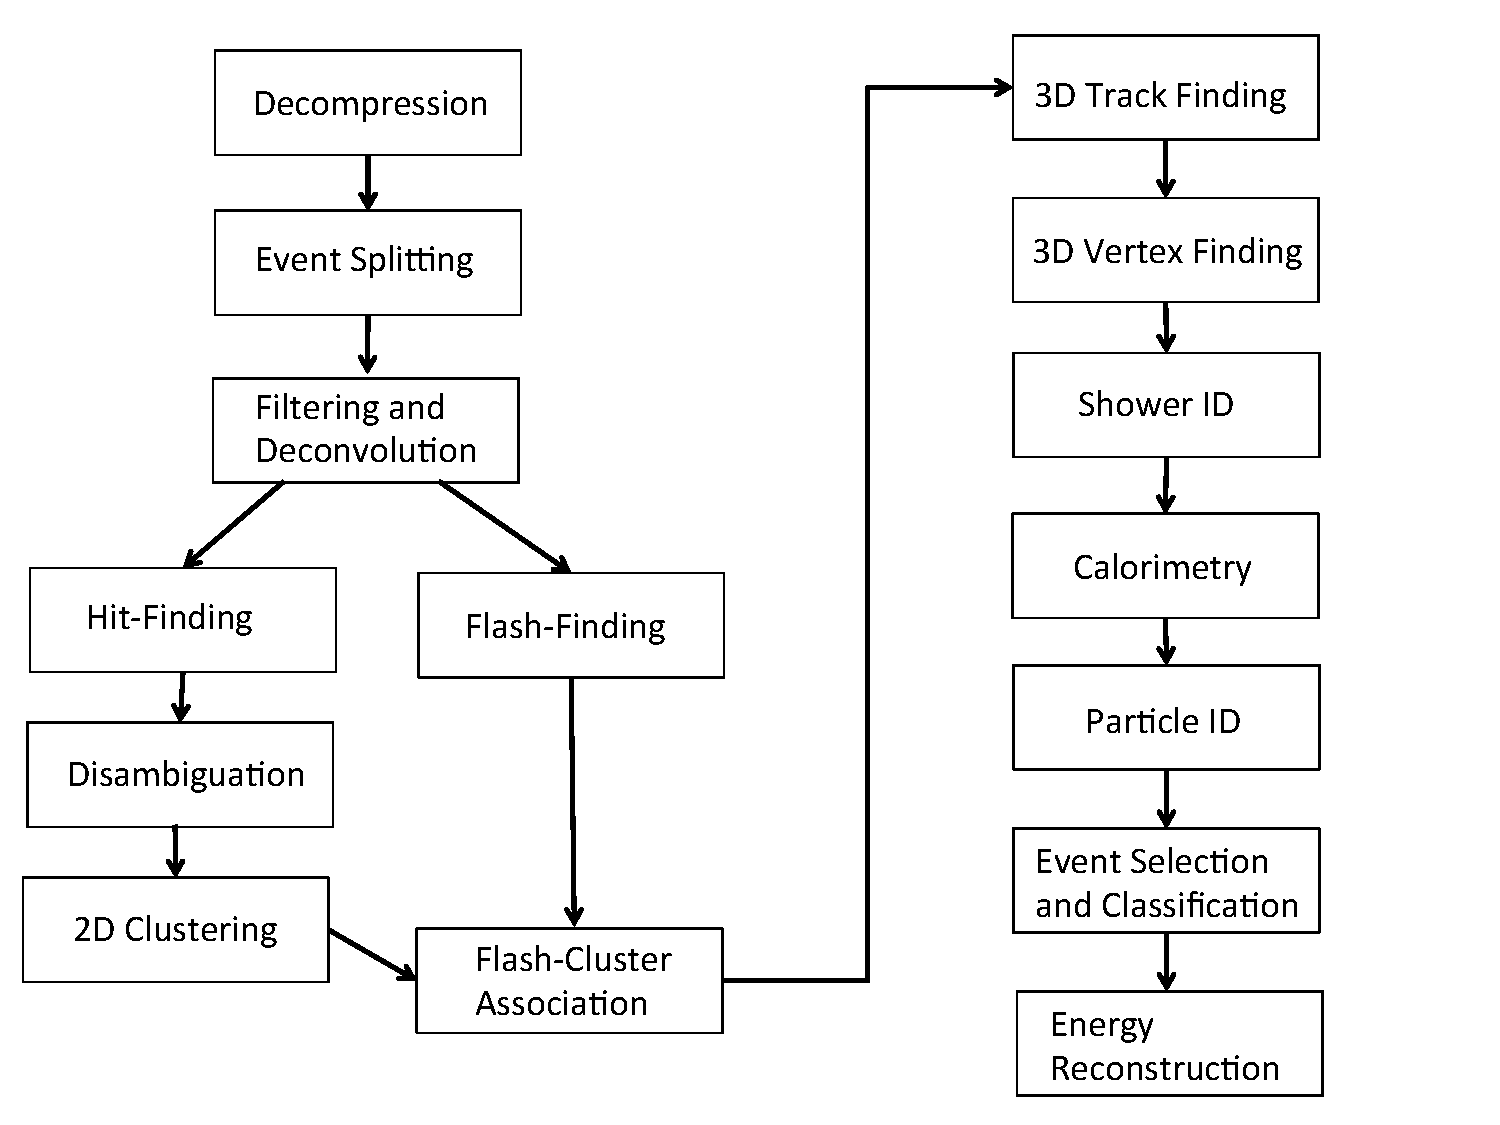
\includegraphics[width=0.7\textwidth]{fdrecoflowchart.pdf}
\end{cdrfigure}


\subsubsection{Signal Processing and Filtering}

The TPC data are first uncompressed and put into local storage, one
channel at a time.  The detector response (bipolar vs. unipolar), and
electronics response functions are deconvoluted using a Fast Fourier
Transform (FFT) algorithm.  The FFT of the data are multiplied by the
inverse of the convolution kernel used in the simulation process,
multiplied by the frequency response of a noise filter, which
suppresses low-frequency and high-frequency noise.  It may be
necessary to filter unipolar signal components on the induction-plane
wires and handle these signals separately, in the case of partial
non-transparency of the induction planes, which might be unavoidable
near the wrapping boundaries.  The product of these is then
inverse-FFT'd back to the time domain to yield the deconvoluted
signals.  A computational speedup is achieved by packing data in
blocks that exceed thresholds plus nearby neighbors in time so that
the FFT only needs to see a fraction of the total ADC samples
collected in each event.

\subsubsection{Flash Finding}


\subsubsection{TPC Hit Finding}

Once deconvoluted, raw ADC values trace out pulses, which are the best
estimates of when charge arrived on a particular electronics channel.
The widths of these pulses are determined by the detector resolution,
by diffusion, and by the intrinsic width of the charge formation
volume projected along the electric field dirction, which can be quite
long in the case of showers or tracks nearly aligned with the electric
field.  Multiple particles may contribute charge to the same pulse,
which is expected to be the case frequently in dense electromagnetic
showers, but can also occur from different particles leaving charge on
segments of the wire that are far apart, as the data from a wire do
not tell where along the wire the charge was deposited, even though
that information is preserved in Monte Carlo simulation files.  Due to
the wrapping of the induction-plane wires, pulses can contain charge
from opposite sides of the APA, but not for collection-plane signals.

Hits are reconstructed pulses on each TPC DAQ channel.  Regions of
interest are identified in the stream of deconvoluted ADC samples, and
sums of Gaussian functions are fitted to the data using
MINUIT~\cite{minuit}.  The peak position, the width, the area, and the
sum of the deconvoluted ADC values corresponding to the fitted
Gaussian are recorded.  In the case that multiple overlapping Gaussian
fits are the best model of the data, the ADC sums are calculated for
the entire region of interest, and then divided among the contributing
hits proportional to their fit areas.  The efficiency of the hit
finder is shown in Figure~\ref{fig:hitfinderefficiency}.

\subsubsection{Disambiguation}

A feature of liquid argon TPC geometries is that the location along a
wire at which charge is deposited is not measured, creating a
one-dimensional continuous ambiguity in the interpretation of the hits
on a wire.  As such, the planes of the TPC read out two-dimensional
``views'' of the three-dimensional events.  The wrapping of the
induction-plane wires in the DUNE APA design introduces another
discrete ambiguity -- the several wire segments that are connected
together to form a DAQ channel all contribute charge on that DAQ
channel, and it is not known from the wire's signal which of those
segments generated the charge.  This discrete ambiguity must be broken
before downstream reconstruction programs can do their work.

The detector geometry is chosen so that no induction-plane wire
crosses any collection-plane wire more than once, necessitating a
shallower induction-plane wire angle of 35.7$^\circ$.  The design from
the LBNE CDR~\cite{lbnecdr} proposed 44.3$^\circ$ and 45.7$^\circ$ as
the angles of the $U$ and $V$ wire planes, which necessitated
associating triplets of $U$, $V$, and $Z$ hits in order to break the
ambiguity.  Hit triplets consistent in drift time and with only one
possible combination of $U$, $V$, and $Z$ hits that intersect in one
position in space are determined to be ``trivially'' disambiguated.
More complicated cases where multiple possible hits in other planes
can be associated with a hit in a given plane, are disambiguated by
looking at nearby unambiguous hits and clustering them together.
Misassociation of hits in the three views, caused mainly by multiple
charge deposits arriving at the same time, can cause choosing the
incorrect wire segment.

The triplet-association algorithm is expected to work very well in the
35.7$^\circ$ geometry, by making few misassociations for the trivially
disambiguated sample.  Figure~\ref{fig:disambig} shows the
disambiguation performance for 6~GeV electrons and muons in the
35.7$^\circ$ far detector geometry.

\subsubsection{Clustering}

% section taken from the LArSoft NIM article -- to rephrase

After hit finding has completed, the hits in each plane are
clustered. The goal of a clustering algorithm is to categorize hits
into individual physics objects as best as possible in 2D. Fuzzy
Cluster is such an algorithm and proceeds in stages, making use of
several algorithms developed outside of
HEP.~\cite{flame}~\cite{ppht}~\cite{dbscan}. These algorithms are
combined to provide a good estimate of which hits can be determined to
come from a single particle.
\subsubsection{Cluster-Flash Association}

\subsubsection{Track-Finding}

% section taken from the LArSoft NIM article -- to rephrase

The track reconstruction problem in a liquid argon TPC can be divided
into several stages, including pattern recognition, identifying hits
that belong to a track, trajectory reconstruction, and track parameter
estimation.

Hits are the input data for track reconstruction.  Hits represent a
one-dimensional measurement of a track (the drift time) on a
measurement surface defined by the charge drift direction and the
readout wire. Hits from multiple views may be combined into
three-dimensional space points. Three dimensional track reconstruction
can proceed from space points or directly from hits.

The Kalman filter algorithm~\cite{kalman} has been widely used in high
energy physics for track reconstruction. The Kalman filter provides an
elegant mathematical solution to the problem of finding an optimal
track description from a collection of candidate measurements that are
hits or space points, especially in cases where the number of
measurements is much larger than the five parameters needed to specify
a track on a surface.  The Kalman filter can be used for both pattern
recognition and parameter estimation.

The measurement surfaces in liquid argon TPCs are intersecting, which
means there is no predetermined order in which the measurement
surfaces should be visited.  To prevent back-and-forth tracking, which
would overestimate propagation noise, such as multiple Coulomb
scattering, the LArSoft Kalman filter chooses the measurement
surfaces associated with one view as primary, and visits these
surfaces in their natural predetermined order.  Hits from views other
than the primary view are added to the track by treating the
propagation from the track surface to the non-parallel hit measurement
surface as part of the measurement function.  This measurement
propagation is always done using a linear approximation as is the
measurement function, and is done without propagation noise.

The LArSoft Kalman filter does not use a branching track model. Hit
selection for the LArSoft Kalman filter is implemented such that at
each measurement surface, the filter accepts either zero or one
hit. If the Kalman filter accepts a wrong hit, the track may follow
the wrong road (e.g. a delta ray), or the track may otherwise end
prematurely.  Fixing broken tracks relies on a track-stitching
algorithm that runs after the initial Kalman filter reconstruction.

\subsubsection{Shower Measurement}

% section taken from the LArSoft NIM article -- to rephrase

The electromagnetic shower reconstruction code happens in two
steps. The first is a post-clustering stage which examines the
existing clusters in terms of their 2D parameters to determine whether
the clusters are shower-like or track-like. The user has the
possibility of refining the existing clusters by additional merging
steps before the final shower-track decision. The selected shower-like
clusters are examined to determine their exact starting point,
direction and angle in the wire-time plane. These parameters are
passed on to the second step, the 3D shower reconstruction code. At
this stage, the 2D clusters are matched between the views to obtain at
least one cluster in two views per tentative shower. These sets of 2D
clusters and their 2D angles and start points are then used to
construct the 3D shower axis and start points via trigonometric
formulae. This allows the calculation of the shower energy and charge
deposition at the start of the shower used in particle
identification. The start point, 3D angle, energy and $dE/dx$ values
are then saved on the event stack for use by an event builder.

\subsubsection{Calorimetry}

% section taken from the LArSoft NIM article -- to rephrase

As charged particles tranverse a volume liquid argon, they deposit
energy through ionization and scintillation. It is important to
measure the energy depotion as it provide information on particle
energy and species. The algorithm for reconstructing the ionization
energy in LArSoft is optimized for line-like tracks and is being
extended to more complicated event topology such as showers. The
algorithm takes all the hits associated with a reconstructed
track. For each hit, the hit area or amplitude, in ADC counts, is
converted to the charge $Q_{det}$, in fC units, on the wire using an
ADC to fC conversion factor that was determined by muons or teststand
measurements. To account for the charge loss along the drift due to
impurities, a first correction is applied to $Q_{det}$ to get the free
charge after recombination $Q_{free} = Q_{det}/e^{-t/\tau_{e}}$, where
$t$ is the electron drift time for the hit and $\tau_{e}$ is the
electron lifetime measured by the muons or purity monitors. The charge
$Q_{free}$ is divided by the track pitch $dx$, which is defined as the
dot production of track direction and the direction normal to the wire
direction in the wire plane, to get the $dQ_{free}/dx$ for the
hit. Finally, to account for charge loss due to recombination, also
known as ``charge quenching'', a second correction is applied to
convert $dQ_{free}/dx$ to $dE/dx$ based on the modified Box's model
\cite{box} or the Birks's model\cite{birks}. The total energy
deposition from the track is obtained by summing the $dE/dx$ from each
hit: $\sum\limits_{i}^{all\ hits}(dE/dx)_{i}\cdot dx_{i}$.


\subsubsection{Particle ID}

% section taken from the LArSoft NIM article -- to rephrase

If the incident particle stops in the LArTPC active volume, the energy
loss, $dE/dx$, as a function of the residual range ($R$), the path
length to the end point of the track, is used as a powerful method for
particle identification. There are two methods in LArSoft to determine
particle species using calorimetric information. The first method
calculates four $\chi^{2}$ values for each track by comparing measured
$dE/dx$ versus $R$ points to the proton, charged kaon, charged pion
and muon hypotheses and identifies the track as the particle that
gives the smallest $\chi^{2}$ value. The second method calculates the
quantity $PIDA = <A_{i}> = <(dE/dx)_{i}R_{i}^{0.42}>$ \cite{box},
which is defined to be the average of $A_{i} =
(dE/dx)_{i}R_{i}^{0.42}$ over all track points where the residual
range $R_{i}$ is less than 30 cm. The particle species can be
determined by making a selection on the $PIDA$ value.

\subsubsection{Calibration}



